
\documentclass[tikz,border=8pt]{standalone}

\usepackage[T1]{fontenc}
\usepackage{lmodern}
\usepackage{xcolor}
\usetikzlibrary{
	arrows.meta,
	positioning,
	shapes.geometric,
	fit,
	backgrounds,
	calc
}

\definecolor{outer}{HTML}{DCEAF7}
\definecolor{outerline}{HTML}{356A9A}
\definecolor{inner}{HTML}{E2F2E9}
\definecolor{innerline}{HTML}{32805B}
\definecolor{hybrid}{HTML}{FFF0D6}
\definecolor{hybridline}{HTML}{B87919}
\definecolor{selectc}{HTML}{EAE3F7}
\definecolor{selectline}{HTML}{7957A6}
\definecolor{neutral}{HTML}{F2F4F7}
\definecolor{neutralline}{HTML}{64748B}

\tikzset{
	process/.style={
		draw=neutralline,
		fill=neutral,
		rounded corners=3pt,
		align=center,
		text width=3.6cm,
		minimum height=0.85cm,
		font=\small,
		inner sep=5pt
	},
	outerbox/.style={
		process, draw=outerline, fill=outer
	},
	innerbox/.style={
		process, draw=innerline, fill=inner
	},
	hybridbox/.style={
		process, draw=hybridline, fill=hybrid
	},
	selectbox/.style={
		process, draw=selectline, fill=selectc
	},
	decision/.style={
		diamond,
		aspect=2.1,
		draw=neutralline,
		fill=neutral,
		align=center,
		text width=2.5cm,
		inner sep=2pt,
		font=\small
	},
	flow/.style={
		-{Stealth[length=2.2mm]},
		thick,
		draw=neutralline
	},
	feedback/.style={
		-{Stealth[length=2mm]},
		semithick,
		dashed,
		draw=neutralline
	}
}

\begin{document}
	
	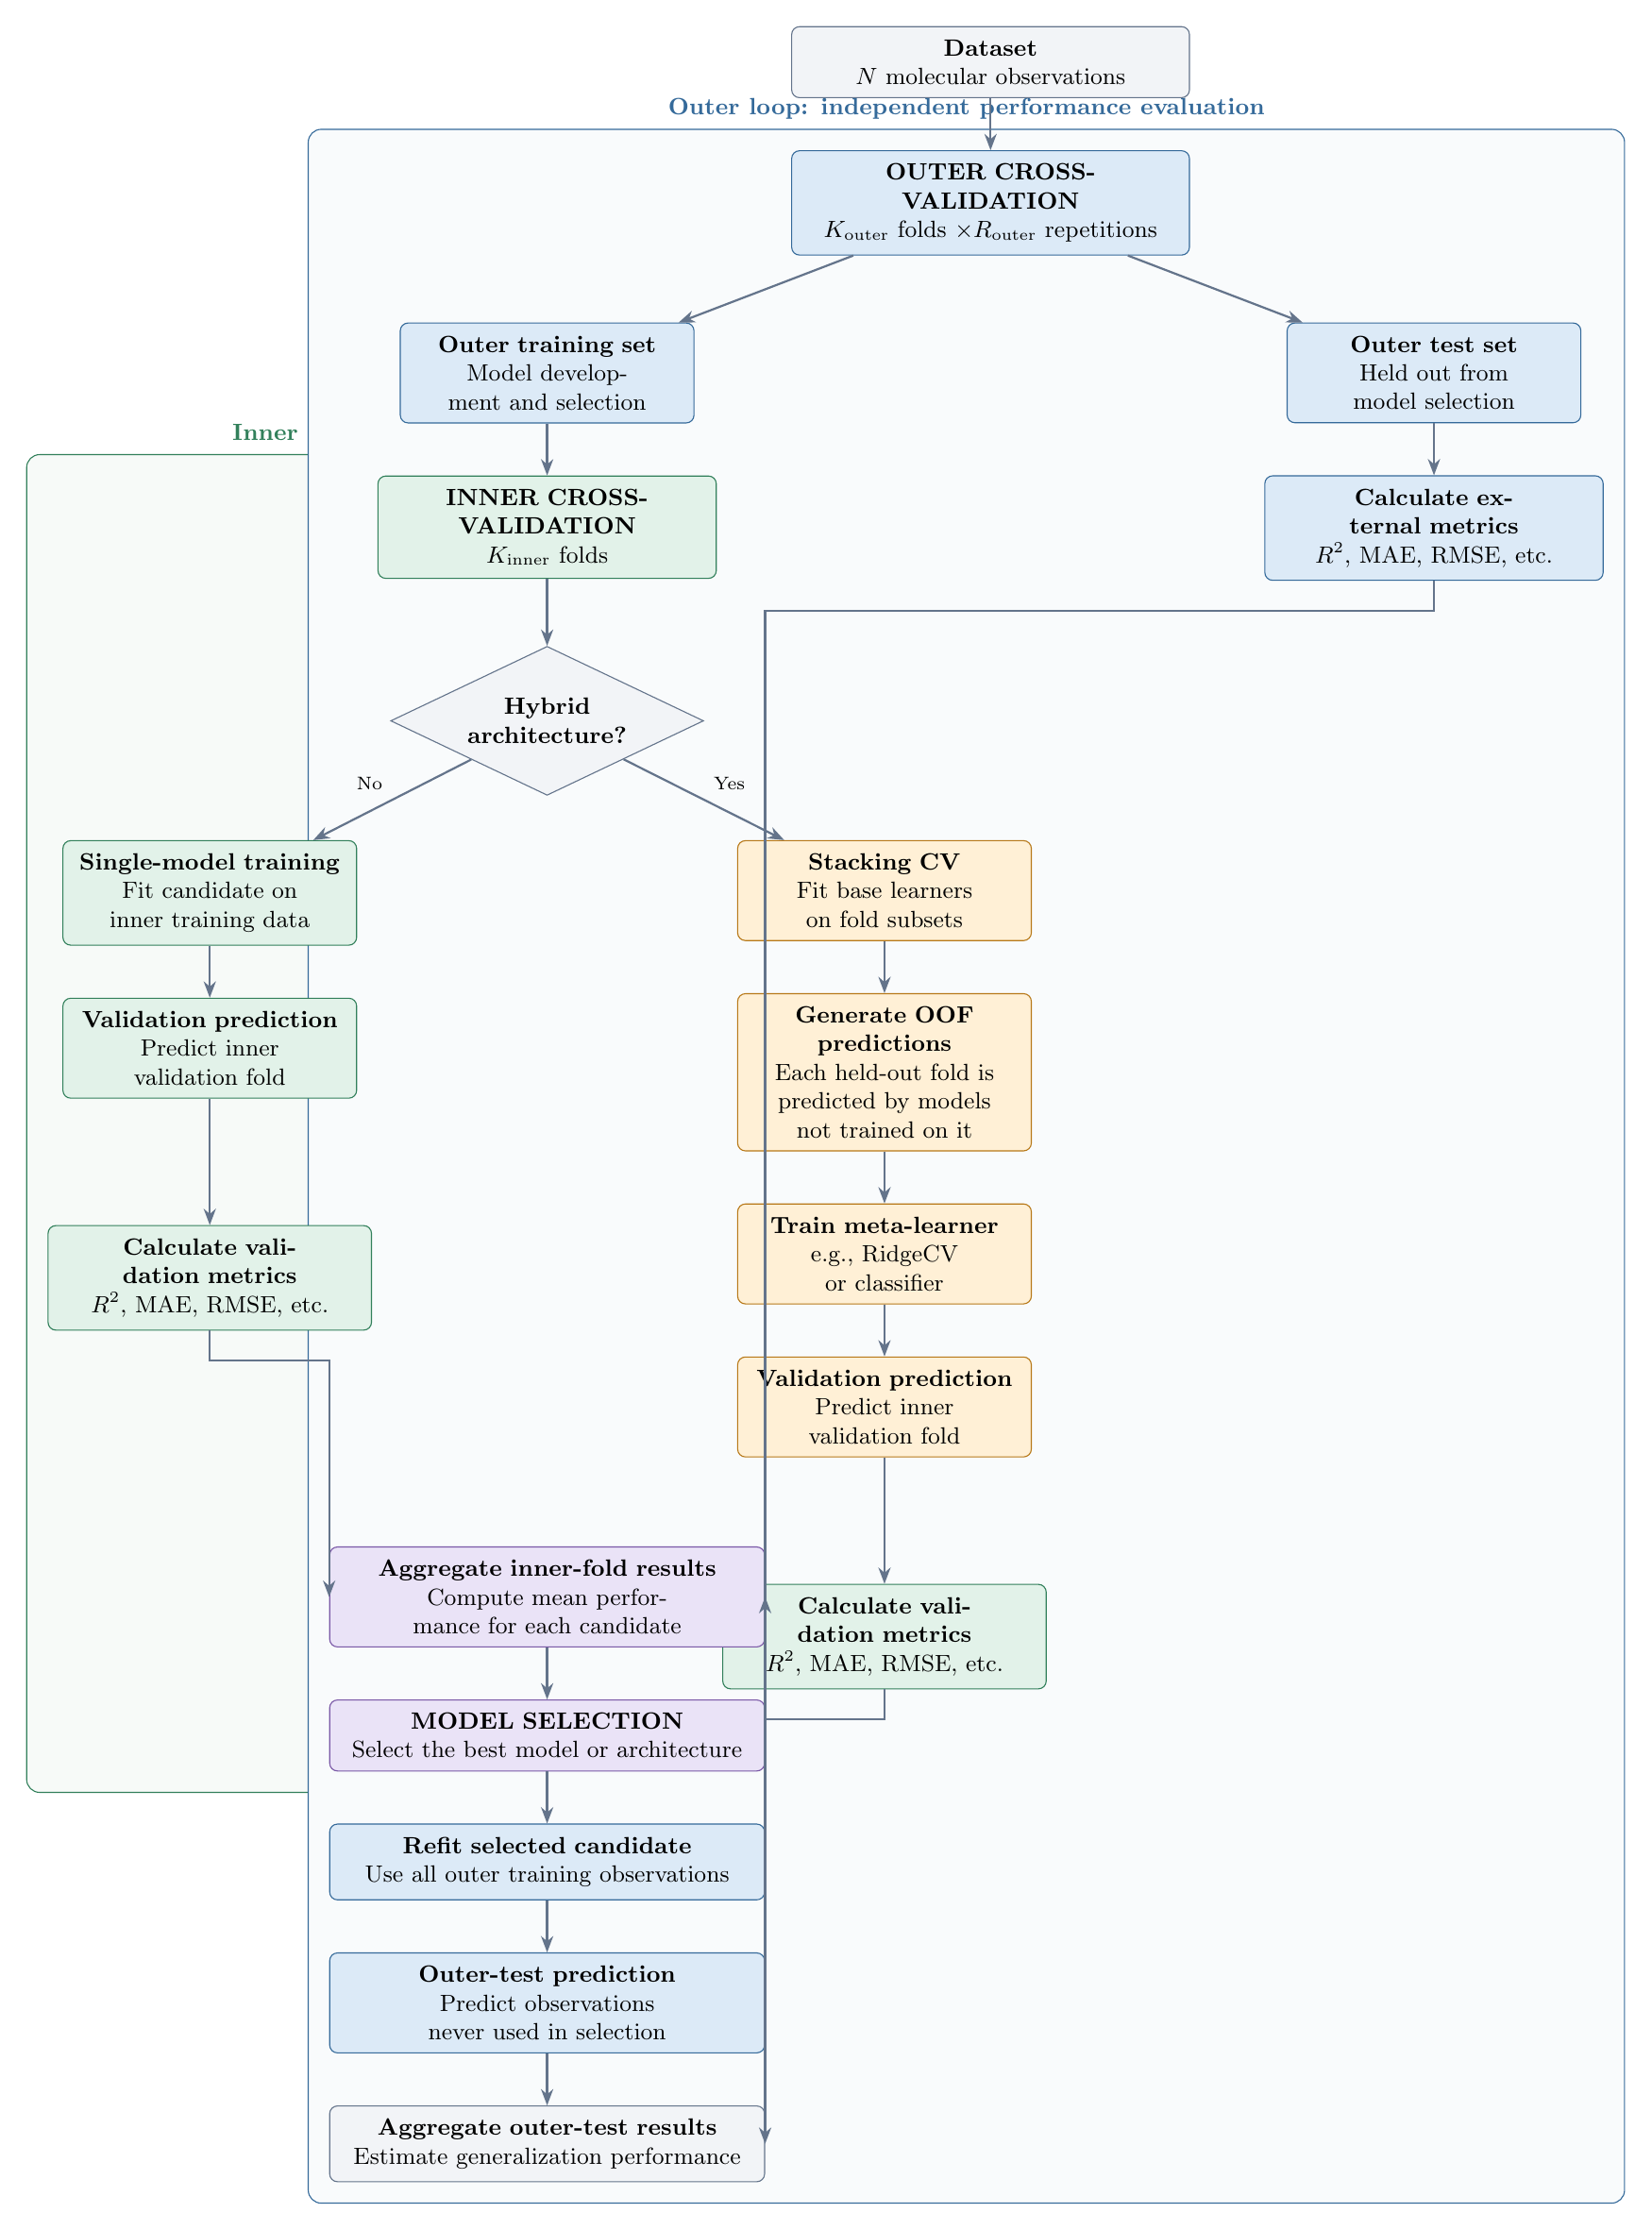
\begin{tikzpicture}[
		node distance=7mm and 10mm
		]
		
		% =================================================
		% OUTER CROSS-VALIDATION
		% =================================================
		
		\node[process, text width=5.0cm] (data) {
			\textbf{Dataset}\\
			$N$ molecular observations
		};
		
		\node[outerbox, below=of data, text width=5.0cm] (outercv) {
			\textbf{OUTER CROSS-VALIDATION}\\
			$K_{\mathrm{outer}}$ folds
			$\times R_{\mathrm{outer}}$ repetitions
		};
		
		\node[outerbox, below left=9mm and 13mm of outercv]
		(outertrain) {
			\textbf{Outer training set}\\
			Model development and selection
		};
		
		\node[outerbox, below right=9mm and 13mm of outercv]
		(outertest) {
			\textbf{Outer test set}\\
			Held out from model selection
		};
		
		\draw[flow] (data) -- (outercv);
		\draw[flow] (outercv) -- (outertrain);
		\draw[flow] (outercv) -- (outertest);
		
		% =================================================
		% INNER CROSS-VALIDATION
		% =================================================
		
		\node[innerbox, below=of outertrain, text width=4.2cm]
		(innercv) {
			\textbf{INNER CROSS-VALIDATION}\\
			$K_{\mathrm{inner}}$ folds
		};
		
		\node[decision, below=9mm of innercv] (decision) {
			\textbf{Hybrid}\\
			\textbf{architecture?}
		};
		
		\draw[flow] (outertrain) -- (innercv);
		\draw[flow] (innercv) -- (decision);
		
		% =================================================
		% BRANCH A: SINGLE MODEL
		% =================================================
		
		\node[innerbox, below left=11mm and 15mm of decision]
		(singletrain) {
			\textbf{Single-model training}\\
			Fit candidate on inner training data
		};
		
		\node[innerbox, below=of singletrain] (singlepred) {
			\textbf{Validation prediction}\\
			Predict inner validation fold
		};
		
		\draw[flow] (decision) --
		node[above left, font=\scriptsize] {No}
		(singletrain);
		\draw[flow] (singletrain) -- (singlepred);
		
		% =================================================
		% BRANCH B: HYBRID / STACKING
		% =================================================
		
		\node[hybridbox, below right=11mm and 15mm of decision]
		(basecv) {
			\textbf{Stacking CV}\\
			Fit base learners on fold subsets
		};
		
		\node[hybridbox, below=of basecv] (oof) {
			\textbf{Generate OOF predictions}\\
			Each held-out fold is predicted
			by models not trained on it
		};
		
		\node[hybridbox, below=of oof] (meta) {
			\textbf{Train meta-learner}\\
			e.g., RidgeCV or classifier
		};
		
		\node[hybridbox, below=of meta] (hybridpred) {
			\textbf{Validation prediction}\\
			Predict inner validation fold
		};
		
		\draw[flow] (decision) --
		node[above right, font=\scriptsize] {Yes}
		(basecv);
		\draw[flow] (basecv) -- (oof);
		\draw[flow] (oof) -- (meta);
		\draw[flow] (meta) -- (hybridpred);
		
		% =================================================
		% INNER VALIDATION AND METRICS
		% =================================================
		
		\node[innerbox, below=17mm of singlepred,
		text width=4.0cm] (singlemetrics) {
			\textbf{Calculate validation metrics}\\
			$R^2$, MAE, RMSE, etc.
		};
		
		\node[innerbox, below=17mm of hybridpred,
		text width=4.0cm] (hybridmetrics) {
			\textbf{Calculate validation metrics}\\
			$R^2$, MAE, RMSE, etc.
		};
		
		\draw[flow] (singlepred) -- (singlemetrics);
		\draw[flow] (hybridpred) -- (hybridmetrics);
		
		% =================================================
		% MODEL SELECTION
		% =================================================
		
		\node[selectbox, below=12mm of $(singlemetrics)!0.5!(hybridmetrics)$,
		text width=5.5cm] (aggregate) {
			\textbf{Aggregate inner-fold results}\\
			Compute mean performance for each candidate
		};
		
		\node[selectbox, below=of aggregate, text width=5.5cm]
		(selection) {
			\textbf{MODEL SELECTION}\\
			Select the best model or architecture
		};
		
		\draw[flow] (singlemetrics.south) --
		++(0,-4mm) -| (aggregate.west);
		
		\draw[flow] (hybridmetrics.south) --
		++(0,-4mm) -| (aggregate.east);
		
		\draw[flow] (aggregate) -- (selection);
		
		% =================================================
		% REFIT AND OUTER EVALUATION
		% =================================================
		
		\node[outerbox, below=of selection, text width=5.5cm]
		(refit) {
			\textbf{Refit selected candidate}\\
			Use all outer training observations
		};
		
		\node[outerbox, below=of refit, text width=5.5cm]
		(outerpredict) {
			\textbf{Outer-test prediction}\\
			Predict observations never used in selection
		};
		
		\node[outerbox, below=of outertest, text width=4.2cm]
		(externalmetrics) {
			\textbf{Calculate external metrics}\\
			$R^2$, MAE, RMSE, etc.
		};
		
		\node[process, below=of outerpredict, text width=5.5cm]
		(finalresults) {
			\textbf{Aggregate outer-test results}\\
			Estimate generalization performance
		};
		
		\draw[flow] (selection) -- (refit);
		\draw[flow] (refit) -- (outerpredict);
		
		\draw[flow] (outertest) -- (externalmetrics);
		
		\draw[flow] (outerpredict) -- (finalresults);
		\draw[flow] (externalmetrics.south) --
		++(0,-4mm) -| (finalresults.east);
		
		% =================================================
		% BACKGROUND GROUPS
		% =================================================
		
		\begin{scope}[on background layer]
			
			\node[
			draw=innerline,
			fill=innerline!4,
			rounded corners=5pt,
			inner sep=8pt,
			fit=(innercv)(decision)(singletrain)(singlepred)
			(basecv)(oof)(meta)(hybridpred)
			(singlemetrics)(hybridmetrics)(aggregate)(selection),
			label={[text=innerline,font=\bfseries\small]
				above:Inner loop: training, validation and model selection}
			] {};
			
			\node[
			draw=outerline,
			fill=outerline!3,
			rounded corners=5pt,
			inner sep=8pt,
			fit=(outercv)(outertrain)(outertest)(refit)
			(outerpredict)(externalmetrics)(finalresults),
			label={[text=outerline,font=\bfseries\small]
				above:Outer loop: independent performance evaluation}
			] {};
			
		\end{scope}
		
	\end{tikzpicture}
\end{document}
